\section{凸共轭}
\label{sec:dual-conjugate}

计算对偶函数时，内层总是“目标加上一个线性项，再取下确界”。线性等式约束$\bm{A}\bm{x}=\bm{b}$的对偶函数就是
\[
 q(\bm{\nu})=\inf_{\bm{x}}\bigl\{f(\bm{x})+\langle\bm{A}^\top\bm{\nu},\bm{x}\rangle\bigr\}-\bm{b}^\top\bm{\nu}.
\]
能否把“$f$加线性项后的下确界”事先算好，以后遇到不同的约束时直接取用？这个运算单独拿出来，就是凸共轭。

\subsection{共轭的定义与计算}
\label{sec:dual-conjugate-definition}

下确界$\inf_{\bm{x}}\{f(\bm{x})+\langle\bm{c},\bm{x}\rangle\}$有一个直观的图景。固定斜率$\bm{y}$，拿一把这个斜率的直尺从下方往上顶，顶到碰到$f$为止。这把直尺就是斜率为$\bm{y}$的最高仿射下界。要求直线$\langle\bm{y},\bm{x}\rangle-\beta$处处不超过$f$，等价于对所有$\bm{x}$有
\[
 \beta\geq\langle\bm{y},\bm{x}\rangle-f(\bm{x}).
\]
最小的$\beta$是右端对$\bm{x}$的上确界，这就是下面的定义。

\begin{definition}[凸共轭]
 \label{def:dual-conjugate}
 设$f:\mathbb{R}^n\to\mathbb{R}\cup\{+\infty\}$是适当函数。它的\term{凸共轭}（convex conjugate）是
 \begin{equation}
  f^*(\bm{y})=\sup_{\bm{x}\in\operatorname{dom}f}\bigl\{\langle\bm{y},\bm{x}\rangle-f(\bm{x})\bigr\},
  \label{eq:dual-conjugate}
 \end{equation}
 取值于$\mathbb{R}\cup\{+\infty\}$。
\end{definition}

记号上要小心，$f^*$是共轭函数，$f^\star$是最优值，两者不是一回事。对固定的$\bm{x}$，$\langle\bm{y},\bm{x}\rangle-f(\bm{x})$是$\bm{y}$的仿射函数，$f^*$是它们的上确界，所以无论$f$是否凸，$f^*$总是凸的。这与定理~\ref{thm:dual-concave}是同一个论证。

图~\ref{fig:dual-conj-tangent}(a)取$f(x)=x^2$，斜率$y=2$。过原点的点线$2x$在$x=1$处比$f$高出最多，这个最大的竖直距离是$1$。把点线向下平移$1$，得到切线$2x-1$，它与竖轴的交点是$-f^*(2)$。所以$f^*(y)$是把斜率$y$的直线降到$f$之下需要降多少。

也可以把$\bm{y}$读成价格，把$f(\bm{x})$读成生产$\bm{x}$的成本，于是$f^*(\bm{y})$是价格$\bm{y}$下能得到的最大利润。这个类比说明了为什么$f^*$对$\bm{y}$是凸的：价格上涨时，厂商可以调整产量，利润的增长比线性更快。类比的边界在于$\bm{x}$可以取负值，$f$也不必是真实的成本。

\begin{BookInlineFigure}
 \centering
 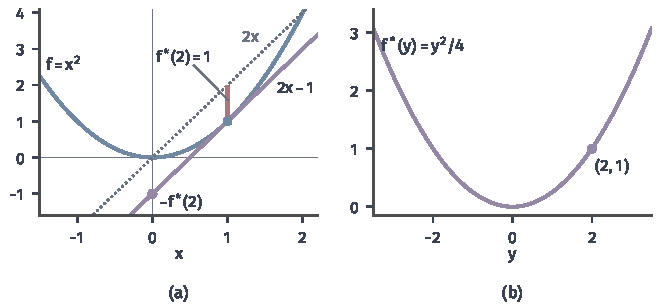
\includegraphics[width=112mm]{figures/05-optimization/06-constrained-optimization/matplotlib/dual-conj-tangent/figure.pdf}
 \caption{共轭是最高仿射下界的截距。(a)~蓝线是$f(x)=x^2$，灰色点线是$y=2$的直线$2x$，红色线段是它与$f$的最大竖直距离$f^*(2)=1$，紫线是下移后的切线，紫点是截距$-f^*(2)$。(b)~紫线是共轭函数$f^*(y)=y^2/4$，紫点对应$y=2$。}
 \label{fig:dual-conj-tangent}
\end{BookInlineFigure}

下面计算三个基本的共轭，每个都要回答一个问题：$f^*$在哪些$\bm{y}$上取有限值。

\paragraph{正定二次函数}
设$\bm{Q}\in\mathbb{R}^{n\times n}$对称正定，$f(\bm{x})=\frac12\bm{x}^\top\bm{Q}\bm{x}$。对$\bm{x}$配方，令$\bm{w}=\bm{x}-\bm{Q}^{-1}\bm{y}$，得到
\[
 \langle\bm{y},\bm{x}\rangle-\frac12\bm{x}^\top\bm{Q}\bm{x}=\frac12\bm{y}^\top\bm{Q}^{-1}\bm{y}-\frac12\bm{w}^\top\bm{Q}\bm{w}.
\]
第二项非正，在$\bm{w}=\bm{0}$时取零，于是
\begin{equation}
 f^*(\bm{y})=\frac12\bm{y}^\top\bm{Q}^{-1}\bm{y}.
 \label{eq:dual-conj-quadratic}
\end{equation}

正定性保证上确界在每个$\bm{y}$上都有限。$f(x)=x^2$相当于$Q=2$，式~\eqref{eq:dual-conj-quadratic}给出$f^*(y)=y^2/4$，$f^*(2)=1$，与图一致。

若$\bm{Q}$只是半正定，$f^*$的有限范围会缩小。例如$\mathbb{R}^2$上的$f(\bm{x})=\frac12x_1^2$，只要$y_2\neq0$，沿$x_2$方向无限走，$\langle\bm{y},\bm{x}\rangle$就趋于$+\infty$，所以$f^*(\bm{y})=+\infty$；只有$y_2=0$时，$f^*(\bm{y})=\frac12y_1^2$。

最极端的情形是线性函数$f(\bm{x})=\langle\bm{a},\bm{x}\rangle$。上确界$\sup_{\bm{x}}\langle\bm{y}-\bm{a},\bm{x}\rangle$只有$\bm{y}=\bm{a}$时有限，此时为$0$。这正是线性规划对偶中出现等式约束的原因。

\paragraph{范数}
设$\lVert\cdot\rVert$是$\mathbb{R}^n$上的一个范数。为了表述结果，先定义它的\term{对偶范数}（dual norm）：
\begin{equation}
 \lVert\bm{y}\rVert_*=\sup_{\lVert\bm{x}\rVert\leq1}\langle\bm{y},\bm{x}\rangle.
 \label{eq:dual-dual-norm}
\end{equation}
由定义，对所有$\bm{x}$，
\[
 \langle\bm{y},\bm{x}\rangle\leq\lVert\bm{y}\rVert_*\lVert\bm{x}\rVert.
\]

现在求$f(\bm{x})=\lVert\bm{x}\rVert$的共轭，分两种情形。若$\lVert\bm{y}\rVert_*\leq1$，由上式，线性项不超过范数，差值不大于零，并在$\bm{x}=\bm{0}$取到零，上确界为$0$。若$\lVert\bm{y}\rVert_*>1$，存在$\lVert\bm{x}_0\rVert\leq1$使$\langle\bm{y},\bm{x}_0\rangle>1$，于是线性项超过范数；沿$s\bm{x}_0$放大，差值随$s$线性增长，趋于$+\infty$。

合起来，范数的共轭是对偶范数单位球的约束指标函数：
\begin{equation}
 f^*(\bm{y})=\iota_{\{\lVert\bm{y}\rVert_*\leq1\}}(\bm{y}).
 \label{eq:dual-conj-norm}
\end{equation}

图~\ref{fig:dual-conj-norm}(a)和(b)是一元情形$f(x)=\lvert x\rvert$。斜率的绝对值不超过$1$的直线都能放在折线下方，斜率$1.5$的直线在$x>0$一侧无论怎样下移，最终都会越过$\lvert x\rvert$。

\paragraph{集合的约束指标函数}
设$\bm{C}$非空。由定义，
\begin{equation}
 \iota_{\bm{C}}^*(\bm{y})=\sup_{\bm{x}\in\bm{C}}\langle\bm{y},\bm{x}\rangle=:\sigma_{\bm{C}}(\bm{y}),
 \label{eq:dual-support}
\end{equation}
$\sigma_{\bm{C}}$称为$\bm{C}$的\term{支撑函数}（support function）。它回答：沿方向$\bm{y}$看，集合最远伸到哪里。集合有界时它处处有限，无界时在某些方向上可能为$+\infty$。

一元的例子是$\bm{C}=[-1,2]$。$y\geq0$时最远点是$2$，$y<0$时最远点是$-1$，所以
\[
 \sigma_{\bm{C}}(y)=\max\{2y,-y\},
\]
这是图~\ref{fig:dual-conj-norm}(c)的折线。

\begin{BookInlineFigure}
 \centering
 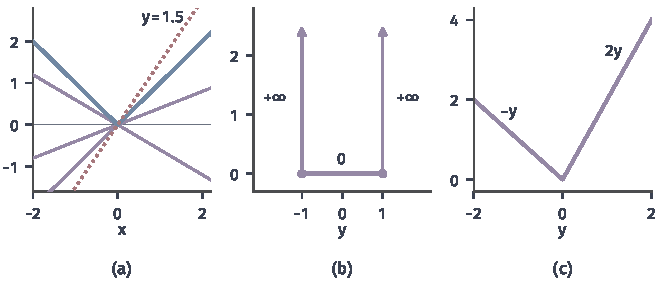
\includegraphics[width=112mm]{figures/05-optimization/06-constrained-optimization/matplotlib/dual-conj-norm/figure.pdf}
 \caption{范数与集合的共轭。(a)~蓝线是$\lvert x\rvert$，紫线是斜率$-0.6,0.4,1$的直线，都在折线下方；红色点线斜率$1.5$，不能下移成下界。(b)~$\lvert x\rvert$的共轭：在$[-1,1]$上为$0$，其余为$+\infty$。(c)~集合$[-1,2]$的支撑函数$\max\{2y,-y\}$。}
 \label{fig:dual-conj-norm}
\end{BookInlineFigure}

二维的例子能同时看到范数和支撑函数的关系。取$\bm{C}$为$\ell_1$单位球，$\bm{y}=(2,1)$。线性函数在多面体上的最大值在顶点取得，比较四个顶点$(\pm1,0),(0,\pm1)$，得到
\[
 \sigma_{\bm{C}}(\bm{y})=\max\{2,-2,1,-1\}=2=\lVert\bm{y}\rVert_\infty.
\]
一般地，$\ell_1$单位球的支撑函数就是$\ell_\infty$范数，也就是说$\ell_1$与$\ell_\infty$互为对偶范数。

图~\ref{fig:dual-support-geometry}(a)中，法向量为$\bm{y}$的直线沿$\bm{y}$方向平移，在$(1,0)$处最后一次碰到菱形。图~\ref{fig:dual-support-geometry}(b)画出了对偶范数的单位球：紫点$(0.6,0.4)$在方块内，线性项处处不超过$\ell_1$范数；红点$(1.4,0.8)$在方块外，取$\bm{x}=(1,0)$，线性项等于$1.4$，超过$\lVert\bm{x}\rVert_1=1$。

\begin{BookInlineFigure}
 \centering
 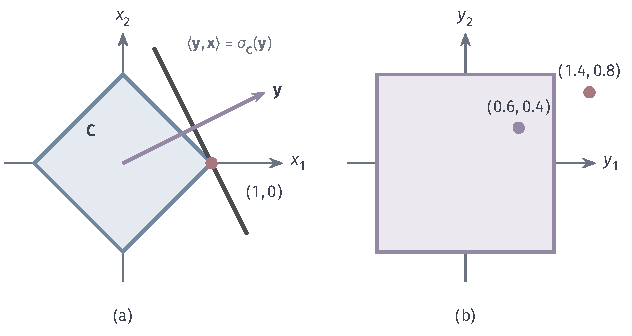
\includegraphics[width=107mm]{figures/05-optimization/06-constrained-optimization/tikz/dual-support-geometry/figure.pdf}
 \caption{支撑函数与对偶范数。(a)~浅蓝菱形是$\ell_1$单位球$\bm{C}$，紫色箭头是方向$\bm{y}=(2,1)$，深灰粗线是在红点$(1,0)$处碰到$\bm{C}$的直线$\langle\bm{y},\bm{x}\rangle=\sigma_{\bm{C}}(\bm{y})=2$。(b)~浅紫方块是$\lVert\bm{y}\rVert_\infty\leq1$，方块内的紫点使共轭为$0$，方块外的红点使共轭为$+\infty$。}
 \label{fig:dual-support-geometry}
\end{BookInlineFigure}

表~\ref{tab:dual-conjugates}汇总了这些结果，并把标量放缩算进去。这些函数常作为作用在辅助变量$\bm{z}$上的惩罚项，所以表中用$\bm{z}$和$\bm{\nu}$作变量。它显示出硬约束与软惩罚在对偶一侧的关系：硬约束$\bm{z}=\bm{0}$的乘子完全自由，二次惩罚让乘子带一个二次代价，范数惩罚让乘子落在一个球内。

\begin{BookInlineTable}
 \centering
 \begin{tabular}{@{}lll@{}}
  \toprule
  原函数$g(\bm{z})$ & 共轭$g^*(\bm{\nu})$ & 有限范围\\
  \midrule
  $\frac{\rho}{2}\lVert\bm{z}\rVert_2^2$（$\rho>0$） & $\frac{1}{2\rho}\lVert\bm{\nu}\rVert_2^2$ & 全空间\\
  $\gamma\lVert\bm{z}\rVert$（$\gamma>0$） & $\iota_{\{\lVert\bm{\nu}\rVert_*\leq\gamma\}}(\bm{\nu})$ & 对偶范数球\\
  $\iota_{\{\bm{0}\}}(\bm{z})$ & $0$ & 全空间\\
  $\iota_{\bm{C}}(\bm{z})$ & $\sigma_{\bm{C}}(\bm{\nu})$ & 由$\bm{C}$决定\\
  $\langle\bm{a},\bm{z}\rangle$ & $\iota_{\{\bm{a}\}}(\bm{\nu})$ & 单点$\bm{a}$\\
  \bottomrule
 \end{tabular}
 \caption{常用函数的共轭。第一行由式~\eqref{eq:dual-conj-quadratic}取$\bm{Q}=\rho\bm{I}$得到，第二行由式~\eqref{eq:dual-conj-norm}放缩得到。}
 \label{tab:dual-conjugates}
\end{BookInlineTable}

\subsection{共轭与最优性}
\label{sec:dual-conjugate-optimality}

共轭除了用来计算，还能描述一个点上的最优性。上确界不小于其中任何一项，由此直接得到一个不等式，它在共轭对偶中的作用，相当于弱对偶在Lagrange对偶中的作用。对任意$\bm{x}\in\operatorname{dom}f$和任意$\bm{y}$，
\begin{equation}
 f(\bm{x})+f^*(\bm{y})\geq\langle\bm{x},\bm{y}\rangle.
 \label{eq:dual-fenchel-young}
\end{equation}
这称为\term{Fenchel--Young不等式}（Fenchel--Young inequality）。

它的几何含义是：直线$\langle\bm{y},\cdot\rangle-f^*(\bm{y})$是$f$的下界，式~\eqref{eq:dual-fenchel-young}是它在$\bm{x}$处的值不超过$f(\bm{x})$。两端的差就是$\bm{x}$处$f$与这条直线之间的竖直距离。图~\ref{fig:dual-fenchel-young}(a)中$f(x)=x^2$，$x=0.5$，$y=2$，差为
\[
 0.25+1-1=0.25.
\]

什么时候取等？第~\ref{chap:nonsmooth-composite-optimization}章定义过次梯度：$\bm{y}\in\partial f(\bm{x})$是指对所有$\bm{x}'$，
\[
 f(\bm{x}')\geq f(\bm{x})+\langle\bm{y},\bm{x}'-\bm{x}\rangle.
\]
这正是说直线在$\bm{x}$处贴着$f$。

\begin{theorem}[Fenchel--Young取等条件]
 \label{thm:dual-fy-equality}
 设$f$是适当的凸函数，$\bm{x}\in\operatorname{dom}f$。则
 \begin{equation}
  \begin{aligned}
   & f(\bm{x})+f^*(\bm{y})=\langle\bm{x},\bm{y}\rangle\\
   \Longleftrightarrow\quad & \bm{y}\in\partial f(\bm{x}).
  \end{aligned}
  \label{eq:dual-fy-equality}
 \end{equation}
\end{theorem}

\begin{proof}
 由定义，左边的等式等价于$\bm{x}$达到式~\eqref{eq:dual-conjugate}中的上确界，也就是对所有$\bm{x}'\in\operatorname{dom}f$，
 \[
  \langle\bm{y},\bm{x}'\rangle-f(\bm{x}')\leq\langle\bm{y},\bm{x}\rangle-f(\bm{x}).
 \]
 移项得到
 \[
  f(\bm{x}')\geq f(\bm{x})+\langle\bm{y},\bm{x}'-\bm{x}\rangle.
 \]
 $\bm{x}'\notin\operatorname{dom}f$时这个不等式自动成立，所以它正是次梯度的定义。
\end{proof}

光滑点上次梯度只有一个，取等的$y$也只有一个，图~\ref{fig:dual-fenchel-young}(a)中$x=1$的切线斜率$2$就是这样。尖点上次梯度有多个，图~\ref{fig:dual-fenchel-young}(b)中$\lvert x\rvert$在$x=0$处，所有$y\in[-1,1]$都取等：
\[
 \lvert0\rvert+f^*(y)=0+0=0\cdot y.
\]

\begin{BookInlineFigure}
 \centering
 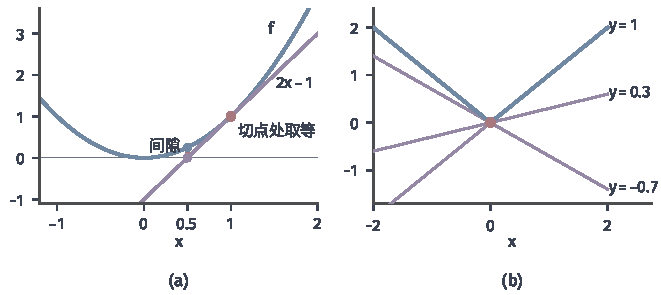
\includegraphics[width=112mm]{figures/05-optimization/06-constrained-optimization/matplotlib/dual-fenchel-young/figure.pdf}
 \caption{Fenchel--Young不等式的几何。(a)~蓝线是$f(x)=x^2$，紫线是$y=2$的最高下界$2x-1$，红色短线是$x=0.5$处的间隙$0.25$，红点$x=1$处间隙为零。(b)~蓝线是$\lvert x\rvert$，紫线是$y=-0.7,0.3,1$的下界，它们都在红点$x=0$处贴着折线，所以这些$y$都是$0$处的次梯度。}
 \label{fig:dual-fenchel-young}
\end{BookInlineFigure}

共轭把$f$变成了一族下方的直线。这些直线够不够重建$f$？把共轭再做一次，得到\term{双共轭}（biconjugate）
\begin{equation}
 f^{**}(\bm{x})=\sup_{\bm{y}}\bigl\{\langle\bm{y},\bm{x}\rangle-f^*(\bm{y})\bigr\},
 \label{eq:dual-biconjugate}
\end{equation}
它是$f$全部仿射下界的上确界。由式~\eqref{eq:dual-fenchel-young}，总有$f^{**}\leq f$。反过来的不等式需要在$f$上方的每个缺口处放进一条直线，工具是分离定理。

\begin{theorem}[点与闭凸集的严格分离]
 \label{thm:dual-separation}
 设$\bm{S}\subseteq\mathbb{R}^N$非空、闭、凸，$\bm{z}\notin\bm{S}$。则存在$\bm{a}\neq\bm{0}$和$\beta\in\mathbb{R}$，使得对所有$\bm{w}\in\bm{S}$，
 \begin{equation}
  \langle\bm{a},\bm{w}\rangle\leq\beta<\langle\bm{a},\bm{z}\rangle.
  \label{eq:dual-separation}
 \end{equation}
\end{theorem}

\begin{proof}
 第~\ref{chap:nonsmooth-composite-optimization}章已得到投影$\bm{p}=\Pi_{\bm{S}}(\bm{z})$的存在性及其刻画：
 \[
  \langle\bm{z}-\bm{p},\bm{w}-\bm{p}\rangle\leq0\qquad\text{对所有}\ \bm{w}\in\bm{S}.
 \]
 令$\bm{a}=\bm{z}-\bm{p}$，$\beta=\langle\bm{a},\bm{p}\rangle$。$\bm{z}\notin\bm{S}$而$\bm{p}\in\bm{S}$，所以$\bm{a}\neq\bm{0}$。上式就是$\langle\bm{a},\bm{w}\rangle\leq\beta$。又因为
 \[
  \langle\bm{a},\bm{z}\rangle=\beta+\lVert\bm{a}\rVert_2^2>\beta,
 \]
 式~\eqref{eq:dual-separation}成立。
\end{proof}

超平面$\{\bm{w}:\langle\bm{a},\bm{w}\rangle=\beta\}$称为\term{分离超平面}（separating hyperplane）。把分离定理用到函数上，要把函数变成集合。函数$f$的\term{上图}（epigraph）是
\[
 \operatorname{epi}f=\{(\bm{x},r):\bm{x}\in\operatorname{dom}f,\ r\geq f(\bm{x})\}.
\]
$f$凸时上图凸。$f$下半连续时上图闭：若$(\bm{x}^{(k)},r^{(k)})\to(\bm{x},r)$且$r^{(k)}\geq f(\bm{x}^{(k)})$，则$r\geq\liminf_kf(\bm{x}^{(k)})\geq f(\bm{x})$。

\begin{theorem}[Fenchel--Moreau]
 \label{thm:dual-fenchel-moreau}
 设$f:\mathbb{R}^n\to\mathbb{R}\cup\{+\infty\}$是适当、下半连续的凸函数，则$f^{**}=f$。
\end{theorem}

\begin{proof}
 已知$f^{**}\leq f$，只需证明：对任意$\bm{x}$和任意实数$r<f(\bm{x})$，存在仿射下界$\ell\leq f$使$\ell(\bm{x})>r$。因为若$\ell(\cdot)=\langle\bm{y},\cdot\rangle-\beta'$是这样的下界，由$\ell\leq f$得$f^*(\bm{y})\leq\beta'$，于是$f^{**}(\bm{x})\geq\ell(\bm{x})>r$。

 点$(\bm{x},r)$不在闭凸集$\operatorname{epi}f$中。对它应用定理~\ref{thm:dual-separation}，并把分离向量取相反数，得到$(\bm{a},b)\neq\bm{0}$和$\beta$，使对所有$(\bm{x}',r')\in\operatorname{epi}f$，
 \[
  \langle\bm{a},\bm{x}'\rangle+br'\geq\beta>\langle\bm{a},\bm{x}\rangle+br.
 \]
 上图沿$r'$向上无界，所以$b\geq0$。

 情形一：$b>0$。取$r'=f(\bm{x}')$并除以$b$，得到仿射下界
 \[
  \ell(\bm{x}')=\frac{\beta-\langle\bm{a},\bm{x}'\rangle}{b}\leq f(\bm{x}'),
 \]
 而分离的严格不等式正是$\ell(\bm{x})>r$。若$\bm{x}\in\operatorname{dom}f$，一定属于这一情形，否则$b=0$时取$\bm{x}'=\bm{x}$，$r'=f(\bm{x})$，得到矛盾：
 \[
  \langle\bm{a},\bm{x}\rangle\geq\beta>\langle\bm{a},\bm{x}\rangle.
 \]

 情形二：$b=0$，此时$\bm{x}\notin\operatorname{dom}f$，并且对所有$\bm{x}'\in\operatorname{dom}f$有$\beta-\langle\bm{a},\bm{x}'\rangle\leq0$。在$\operatorname{dom}f$中任取一点用情形一，得到某个仿射下界$\ell_0\leq f$。对$\varepsilon>0$令
 \[
  \ell_\varepsilon(\bm{x}')=\ell_0(\bm{x}')+\frac{\beta-\langle\bm{a},\bm{x}'\rangle}{\varepsilon}.
 \]
 在$\operatorname{dom}f$上第二项非正，所以$\ell_\varepsilon\leq f$。在点$\bm{x}$处$\beta-\langle\bm{a},\bm{x}\rangle>0$，$\varepsilon$足够小时$\ell_\varepsilon(\bm{x})>r$。
\end{proof}

定理的三个条件各有作用。图~\ref{fig:dual-biconjugate}(a)和(b)说明闭性的作用。$f=\iota_{(0,1)}$是凸函数，但不是下半连续的，因为端点处函数值跳到$+\infty$。它的共轭和双共轭分别是
\[
 f^*(y)=\sup_{0<x<1}xy=\max\{y,0\},\qquad f^{**}=\iota_{[0,1]}.
\]
双共轭补上了两个端点，因为仿射下界分辨不出开区间和它的闭包。

凸性的作用见图~\ref{fig:dual-biconjugate}(c)。双井函数$(x^2-1)^2$的双共轭在$[-1,1]$上是$0$，中间的鼓包被抹平了。一般地，只要$f$有仿射下界，$f^{**}$就是$f$的最大的下半连续凸下界，仿射下界只能看到函数的凸的部分。

\begin{BookInlineFigure}
 \centering
 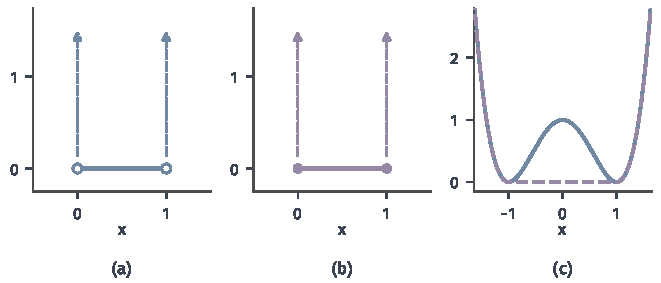
\includegraphics[width=112mm]{figures/05-optimization/06-constrained-optimization/matplotlib/dual-biconjugate/figure.pdf}
 \caption{双共轭恢复什么。(a)~$\iota_{(0,1)}$，两端的空心点表示不属于有效定义域，虚线箭头表示区间外为$+\infty$。(b)~它的双共轭$\iota_{[0,1]}$，端点变为实心。(c)~蓝线是双井函数$(x^2-1)^2$，紫色虚线是数值计算的双共轭，在$[-1,1]$上为零，在外侧与原函数重合。}
 \label{fig:dual-biconjugate}
\end{BookInlineFigure}

定理~\ref{thm:dual-fenchel-moreau}说的是一个函数可以由它的仿射下界重建，并没有说某个约束问题的对偶间隙为零。后者涉及目标和约束的联合结构，要到下一节才能回答，两件事不能混淆。

\subsection{对偶形式的推导}
\label{sec:dual-forms}

有了共轭，对偶函数可以按公式写出，不必每次重新配方。先看线性等式约束$\bm{A}\bm{x}=\bm{b}$，其中$\bm{A}\in\mathbb{R}^{p\times n}$。把内层的线性项按定义~\eqref{eq:dual-conjugate}改写：
\[
 \inf_{\bm{x}}\bigl\{f(\bm{x})+\langle\bm{A}^\top\bm{\nu},\bm{x}\rangle\bigr\}=-\sup_{\bm{x}}\bigl\{\langle-\bm{A}^\top\bm{\nu},\bm{x}\rangle-f(\bm{x})\bigr\}.
\]
右端的上确界是$f^*(-\bm{A}^\top\bm{\nu})$，于是
\begin{equation}
 q(\bm{\nu})=-f^*(-\bm{A}^\top\bm{\nu})-\bm{b}^\top\bm{\nu}.
 \label{eq:dual-q-conj}
\end{equation}

符号要逐项记住：共轭的自变量带负号，因为$\inf$变$\sup$时线性项反号。式~\eqref{eq:dual-q-conj}有限的条件是$-\bm{A}^\top\bm{\nu}\in\operatorname{dom}f^*$，也就是说，共轭的有限范围就是对偶问题的隐含约束。

用二次例核对。$\bm{Q}=\operatorname{diag}(1,4)$，$\bm{A}=(1,1)$，$b=1$。由式~\eqref{eq:dual-conj-quadratic}，
\[
 f^*(-\nu,-\nu)=\frac12\Bigl(\nu^2+\frac{\nu^2}{4}\Bigr)=\frac58\nu^2.
\]
代入式~\eqref{eq:dual-q-conj}得到$q(\nu)=-\frac58\nu^2-\nu$，与式~\eqref{eq:dual-quad-q}相同。

\paragraph{复合形式}
第~\ref{chap:nonsmooth-composite-optimization}章常见的目标是两部分之和，一部分作用在$\bm{x}$上，另一部分作用在$\bm{A}\bm{x}$上：
\begin{equation}
 \min_{\bm{x}}\ F(\bm{x})=f(\bm{x})+g(\bm{A}\bm{x}),
 \label{eq:dual-composite}
\end{equation}
其中$g:\mathbb{R}^p\to\mathbb{R}\cup\{+\infty\}$是一个函数，不是约束函数$g_i$，$\bm{A}\in\mathbb{R}^{p\times n}$。这个问题没有显式的约束，直接写Lagrange函数得不到任何东西。

办法是人为造出一条约束：引入辅助变量$\bm{z}=\bm{A}\bm{x}$，把问题改写成
\[
 \min_{\bm{x},\bm{z}}\ f(\bm{x})+g(\bm{z})\quad\text{s.t.}\quad\bm{A}\bm{x}-\bm{z}=\bm{0}.
\]
这是等价改写，最优值不变。给等式配乘子$\bm{\nu}\in\mathbb{R}^p$，Lagrange函数按$\bm{x}$和$\bm{z}$分成两部分：
\[
 \mathcal{L}=\bigl[f(\bm{x})+\langle\bm{A}^\top\bm{\nu},\bm{x}\rangle\bigr]+\bigl[g(\bm{z})-\langle\bm{\nu},\bm{z}\rangle\bigr].
\]

两部分的下确界可以分别取。第一部分和前面相同，第二部分由共轭的定义得到：
\[
 \inf_{\bm{x}}\bigl[f(\bm{x})+\langle\bm{A}^\top\bm{\nu},\bm{x}\rangle\bigr]=-f^*(-\bm{A}^\top\bm{\nu}),\qquad
 \inf_{\bm{z}}\bigl[g(\bm{z})-\langle\bm{\nu},\bm{z}\rangle\bigr]=-g^*(\bm{\nu}).
\]
于是得到\term{Fenchel对偶}（Fenchel duality）：
\begin{equation}
 \max_{\bm{\nu}}\ q(\bm{\nu})=-f^*(-\bm{A}^\top\bm{\nu})-g^*(\bm{\nu}).
 \label{eq:dual-fenchel}
\end{equation}

图~\ref{fig:dual-composite-flow}是这个推导的结构。注意$\bm{\nu}$在两项里符号相反，这是从$\bm{A}\bm{x}-\bm{z}$的两个系数来的：换成$\bm{z}-\bm{A}\bm{x}$，等于把$\bm{\nu}$换成$-\bm{\nu}$，最优值不变。

\begin{BookInlineFigure}
 \centering
 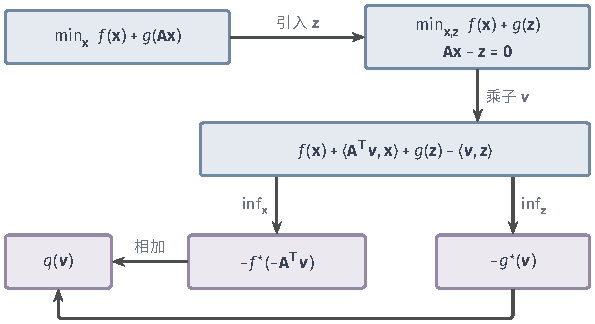
\includegraphics[width=100.8mm]{figures/05-optimization/06-constrained-optimization/tikz/dual-composite-flow/figure.pdf}
 \caption{复合问题的对偶形式怎样得到。浅蓝框是原变量一侧的表达，浅紫框是对偶一侧的量：引入$\bm{z}$，配乘子$\bm{\nu}$，再对$\bm{x}$和$\bm{z}$分别取下确界，得到两个共轭。}
 \label{fig:dual-composite-flow}
\end{BookInlineFigure}

式~\eqref{eq:dual-fenchel}的弱对偶也可以直接从Fenchel--Young不等式看出。对任意$\bm{x}$和$\bm{\nu}$，把式~\eqref{eq:dual-fenchel-young}分别用于$(f,\bm{x},-\bm{A}^\top\bm{\nu})$和$(g,\bm{A}\bm{x},\bm{\nu})$，得到
\[
 f(\bm{x})+f^*(-\bm{A}^\top\bm{\nu})\geq-\langle\bm{A}\bm{x},\bm{\nu}\rangle,\qquad
 g(\bm{A}\bm{x})+g^*(\bm{\nu})\geq\langle\bm{A}\bm{x},\bm{\nu}\rangle.
\]
两式相加，右端抵消，即得$F(\bm{x})\geq q(\bm{\nu})$。

下面算一个例子，目标沿用预算例的二次项，第二项换成绝对值惩罚：
\[
 \min_{\bm{x}\in\mathbb{R}^2}\ \frac12\bigl[(x_1-2)^2+(x_2-1)^2\bigr]+\lvert x_1+x_2\rvert.
\]
这里$\bm{A}=(1,1)$，$g=\lvert\cdot\rvert$，$\bm{a}=(2,1)$，$f(\bm{x})=\frac12\lVert\bm{x}-\bm{a}\rVert_2^2$。

先求$f^*$。上确界的驻点是$\bm{x}=\bm{a}+\bm{y}$，代入得到
\[
 f^*(\bm{y})=\langle\bm{y},\bm{a}\rangle+\frac12\lVert\bm{y}\rVert_2^2.
\]
取$\bm{y}=-\bm{A}^\top\nu=(-\nu,-\nu)$，有
\[
 f^*(-\bm{A}^\top\nu)=-3\nu+\nu^2.
\]

由表~\ref{tab:dual-conjugates}，$g^*=\iota_{[-1,1]}$，它的作用是把$\nu$限制在$[-1,1]$内。于是对偶问题是
\[
 \max_{-1\leq\nu\leq1}\ 3\nu-\nu^2.
\]
无约束最大点$\nu=3/2$在区间外，所以$\nu^\star=1$，对偶值是$3-1=2$。

回到原变量。由$\bm{x}$的驻定条件$\bm{x}-\bm{a}+\bm{A}^\top\nu=\bm{0}$，得到
\[
 \bm{x}=\bm{a}-\bm{A}^\top\nu^\star=(1,0).
\]
核对目标值：$F(1,0)=\frac12(1+1)+1=2$，等于对偶值。根据弱对偶，$(1,0)$是最优解。这里零间隙是算出来的；一般情况下式~\eqref{eq:dual-fenchel}只建立了对偶的表达，零间隙能否成立，要看下一节的条件。
